\section{Zielsetzung}
\label{sec:Zielsetzung}
Ziel des Versuches ist es, die Funktionsweise des He-Ne-Lasers kennenzulernen.

\section{Theorie}
\label{sec:Theorie}

Laser steht für \textbf{L}ight \textbf{A}mplification by \textbf{S}timulated \textbf{E}mission of \textbf{R}adiation, also
Verstärkung des Lichts durch angeregte Emission von Strahlung.
Laser sind demnach Quellen elektromagnetischer Strahlung, die kohärentes, monochromatisches Licht mit einer hohen Intensität aussenden.

%\subsection{Prinzip der Laserstrahlung} % (fold)
%\label{sub:Prinzip}

Ein Laser besteht grundsätzlich aus drei verschiedenen Komponenten, dem aktiven Medium, der Pumpquelle und dem Resonator.
Dies ist schematisch in \autoref{fig:Laserschema} dargestellt.\\

\begin{figure}[H]
    \centering
    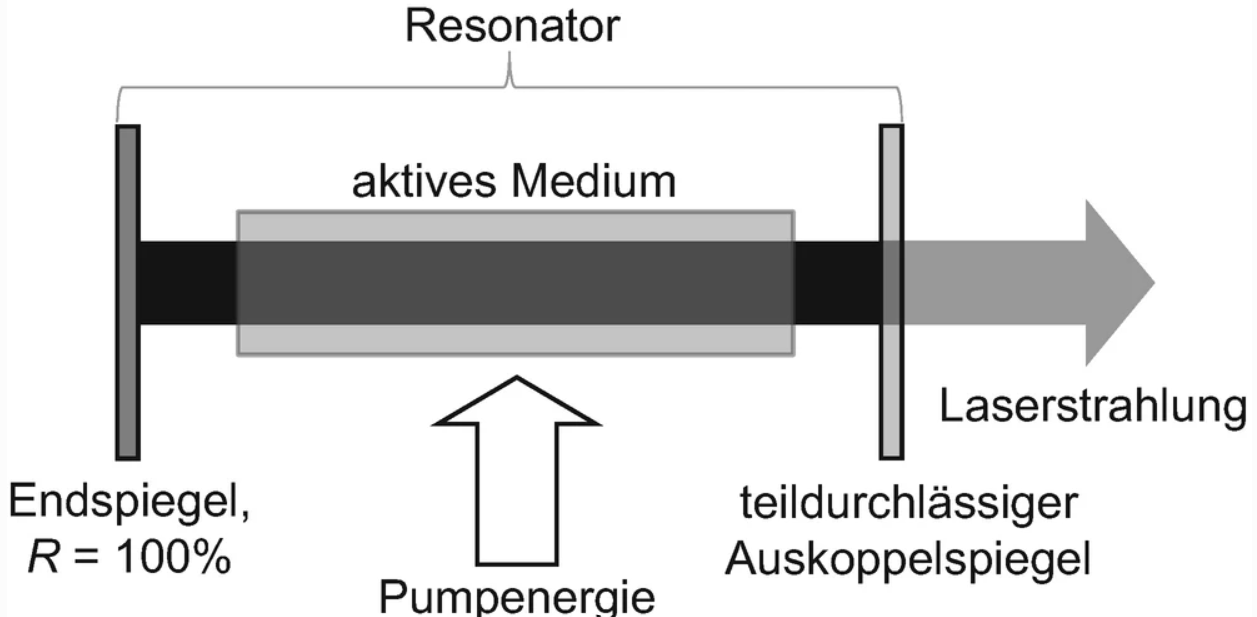
\includegraphics[scale=0.7]{Abbildungen/schemalaser.png}
    \caption{Schematische Aufbau des Lasers.\cite{Gerhard2020}}
    \label{fig:Laserschema}
\end{figure}

Das aktive Medium bestimmt das Strahlungsspektrum und besteht beim He-Ne-Laser aus Neon.
Bei genügend Energiezufuhr durch die Energiepumpe wird im Medium eine Besetzungsinversion der Zustände und eine Lichtverstärkung erreicht.
Besetzungsinversion bedeutet, dass sich mehr Atome im angeregten als im Grundzustand befinden.
Der Resonator dient dazu, den Lichtstrahl mehrfach durch das aktive Medium zu schicken und somit verstärkt eine im Folgenden erläuterte
induzierte Emission der Photonen zu erzwingen.
Wenn die Verstärkung im Resonator gegenüber den Verlusten überwiegt, tritt Lasertätigkeit auf.\\

Lasertätigkeit resultiert aus Wechselwirkungen von Licht mit den Atomen des aktiven Mediums.
Zur vereinfachten Darstellung wird ein Zwei-Niveau-System eines Atoms im Lasermedium angenommen.
Im thermischen Geichgewicht überwiegt die Besetzung des Grundzustands über der des angeregten Zustands nach der Maxwell-Boltzmann-Verteilung.
Wenn ein Photon mit der Energie $E_2-E_1 =\hbar \omega_{12}$ auf ein Atom trifft, hebt es ein Elektron aus einem Energieniveau $E_1$ in ein höheres
Energieniveau $E_2$ an. Das Photon wird dabei absorbiert.
Die spontane Emission beschreibt den umgekehrten Vorgang. Ein angeregtes Atom fällt nach einiger Zeit ohne äußere Einwirkung in den Grundzustand zurück
und emittiert dabei ein Photon. Die Emission dieser Photonen erfolgt gleichmäßig in alle Richtungen.
Die Emission eines Photons kann jedoch nicht nur spontan, sondern auch durch äußere Einwirkung also das Eintreffen eines weiteren Photons
stattfinden. Hierbei besitzt das emittierte Photon dieselbe Frequenz, Phase und Richtung wie das einfallende Photon.
Der Lichtstrahl ist somit kohärent.
Die drei erläuterten Vorgänge sind in \autoref{fig:Strahlungsübergänge} schematisch dargestellt.\\

\begin{figure}[H]
    \centering
    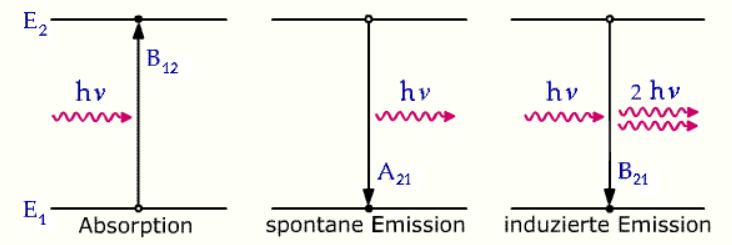
\includegraphics[scale=0.7]{Abbildungen/Prozesse.png}
    \caption{Strahlungsübergänge in einem Zwei-Niveau-System.\cite{prozess}}
    \label{fig:Strahlungsübergänge}
\end{figure}
Die Einsteinkoeffizienten $A_{21}, B_{12}$ und $B_{21}$ sind dabei ein Maß für die Übergangswahrscheinlichkeit.
Die Stärke der verschiedenen Prozesse hängt von der Besetzungszahl $n_i$ im jeweiligen Energiezustand $E_i$ ab.
Bei der induzierten Emission spielt außerdem die Energiedichte $\rho(\nu)$ eine Rolle.

Im beschriebenen Zwei-Niveau-System ist eine Besetzungsinversion nicht möglich, da sich ein Gleichgewichtszustand einstellen würde.
Daher muss ein mindestens Drei-Niveau-System vorliegen, um eine Besetzungsinversion und somit Lasertätigkeit zu ermöglichen.

Ein Resonator gilt als stabil, wenn die auftretenden Verluste kleiner sind als die Verstärkung des Lichtstrahls.
Dies kann über die Stabilitätsbedingung
\begin{align}
    0 \leq g_1 g_2 &< 1 & \text{mit}& & g_i = 1 - \frac{L}{r_i} \label{eqn:Stabilitätsbedingung}
\end{align}
überprüft werden, wobei $g_i$ die Spiegelparameter mit den Krümmungsradien $r_i$ und der Resonatorlänge $L$ darstellen.

Es bilden sich im Laser mehrere Moden, also stehende Wellen. Dabei sind die Moden eine stationäre Feldverteilung. Sie werden als TEm$_{lqp}$-Moden bezeichnet, wobei das $l$ und $p$ für die 
transversalen Moden stehen und das $q$ für die longitudinalen Moden. Die transversalen Moden sind Schwingungen senkrecht zur Ausbreitungsrichtung und die longitudinalen Moden sind
Schwingungen parallel zur Ausbreitungsrichtung, die zum Beispiel durch Unebenheiten an den Spiegeln entstehen. Die Grundmode ist die TEM$_{00}$-Mode, welche eine Intensität von 
\begin{align*}
    I(r) = I_0 \text{exp}(\frac{-2r^2}{\omega^2})
\end{align*}
besitzt. Moden, die höher als die Grundmode sind, werden als Multimoden bezeichnet. Diese führen zu unregelmäßiger Lichtintensität im Strahlprofil und schlechterer Strahlqualität.




